

%%
%% Benchmarks
%%



\begin{frame}{Benchmarks}

 \begin{center}
   {\Large \textbf{Which approach is fastest?}} \\[1em]
%    \includegraphics[width=0.6\textwidth]{figures/race33} \\
%  \tiny http://www.you-can-be-funny.com/images/race33.jpg \\[3em]
 
 {\footnotesize Sorted vs. Scalable vs. Scalable, fast vs. Heap vs. BTHeap vs. \\
 Linked-list condensed vs. RowMerge vs. RowMerge2 }
 \end{center}

\end{frame}

\begin{frame}{Benchmark Results}
\begin{block}{Comparison of Sequential MatMatMult in PETSc}
 \begin{center}
  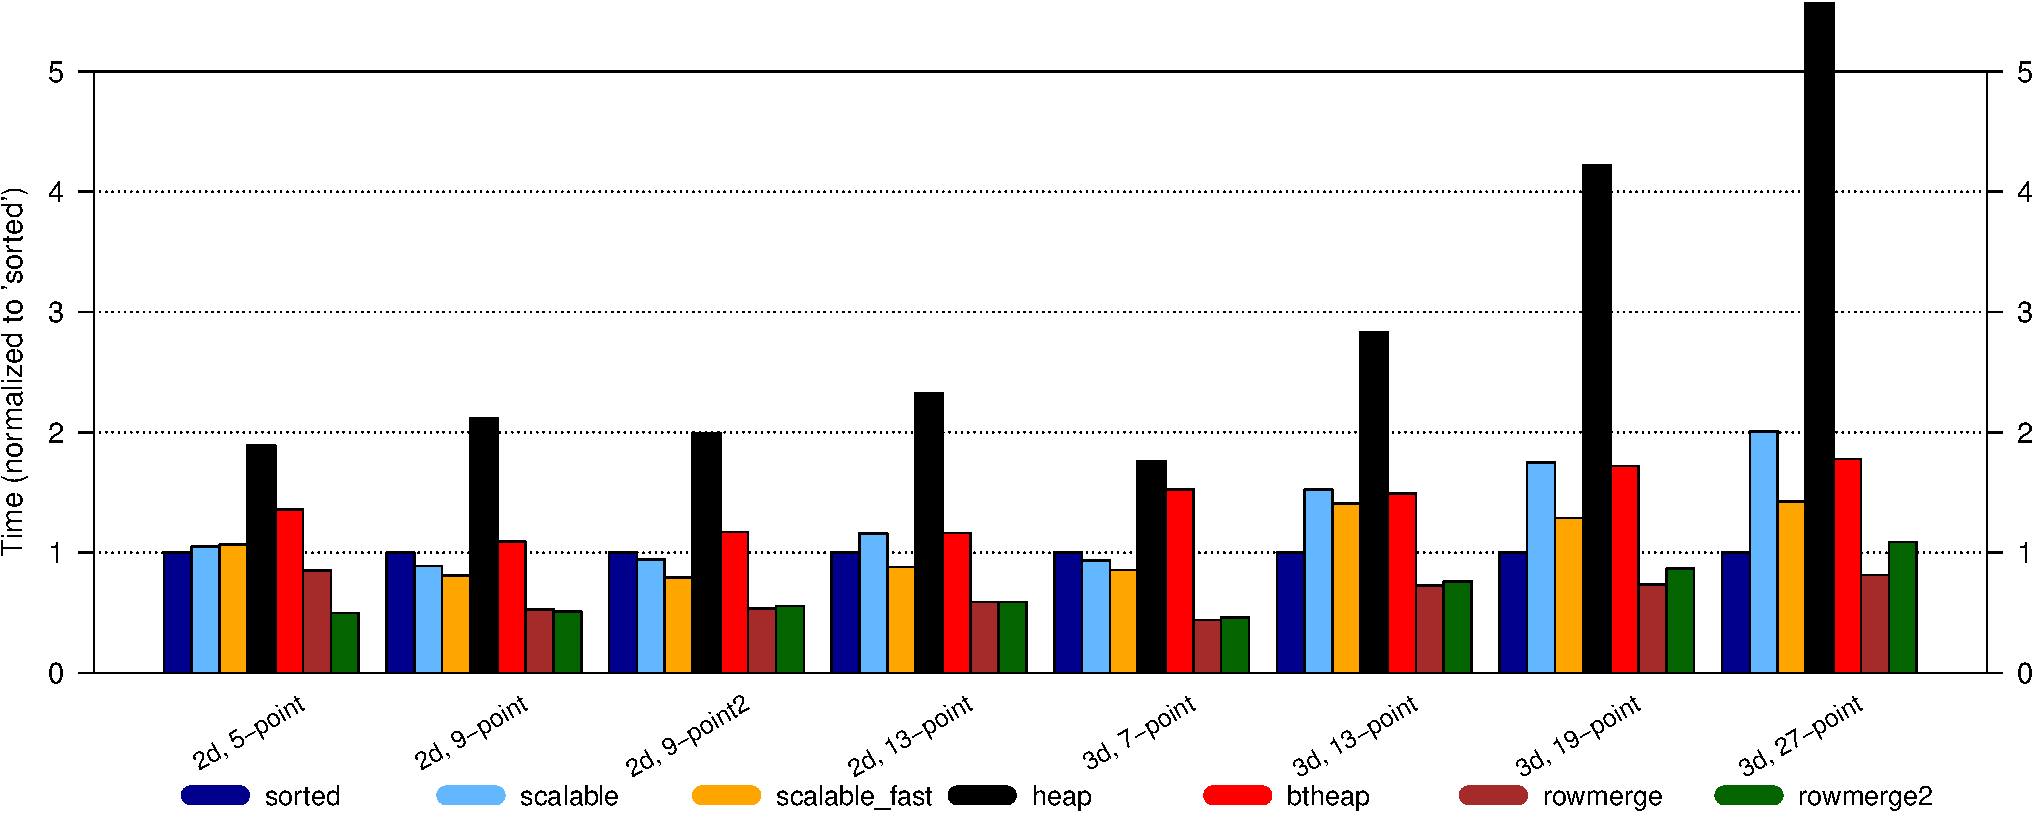
\includegraphics[width=0.999\textwidth]{figures/petsc-matmatmult-crop} \\[1em]
  {\scriptsize (Tests run on an Intel Core i3-3217U)}
 \end{center}
 \begin{itemize}
  \item Row Merge up to 2x faster than PETSc's default
 \end{itemize}
\end{block}
\end{frame}



\begin{frame}{Benchmark Setup}

 \begin{block}{Hardware for Comparison}
  \begin{itemize}
   \item AMD FirePro W9100 GPU
   \item Intel Xeon E5-2670v3 (Haswell, dual socket)
   \item NVIDIA Tesla K20
  \end{itemize}
 \end{block}

  \begin{block}{Software for Comparison}
  \begin{itemize}
   \item Intel MKL 11.2.1
   \item NVIDIA cuSPARSE 7.0
   \item CUSP 0.5.1
  \end{itemize}
 \end{block}

 \begin{block}{Matrices}
  \begin{itemize}
   \item 20 matrices from Florida Sparse Matrix Collection
   \item Operation: $\mathbf{B} = \mathbf{A}\mathbf{A}$
  \end{itemize}
 \end{block}

\end{frame}


\begin{frame}{Benchmark Results}
 \begin{center}
  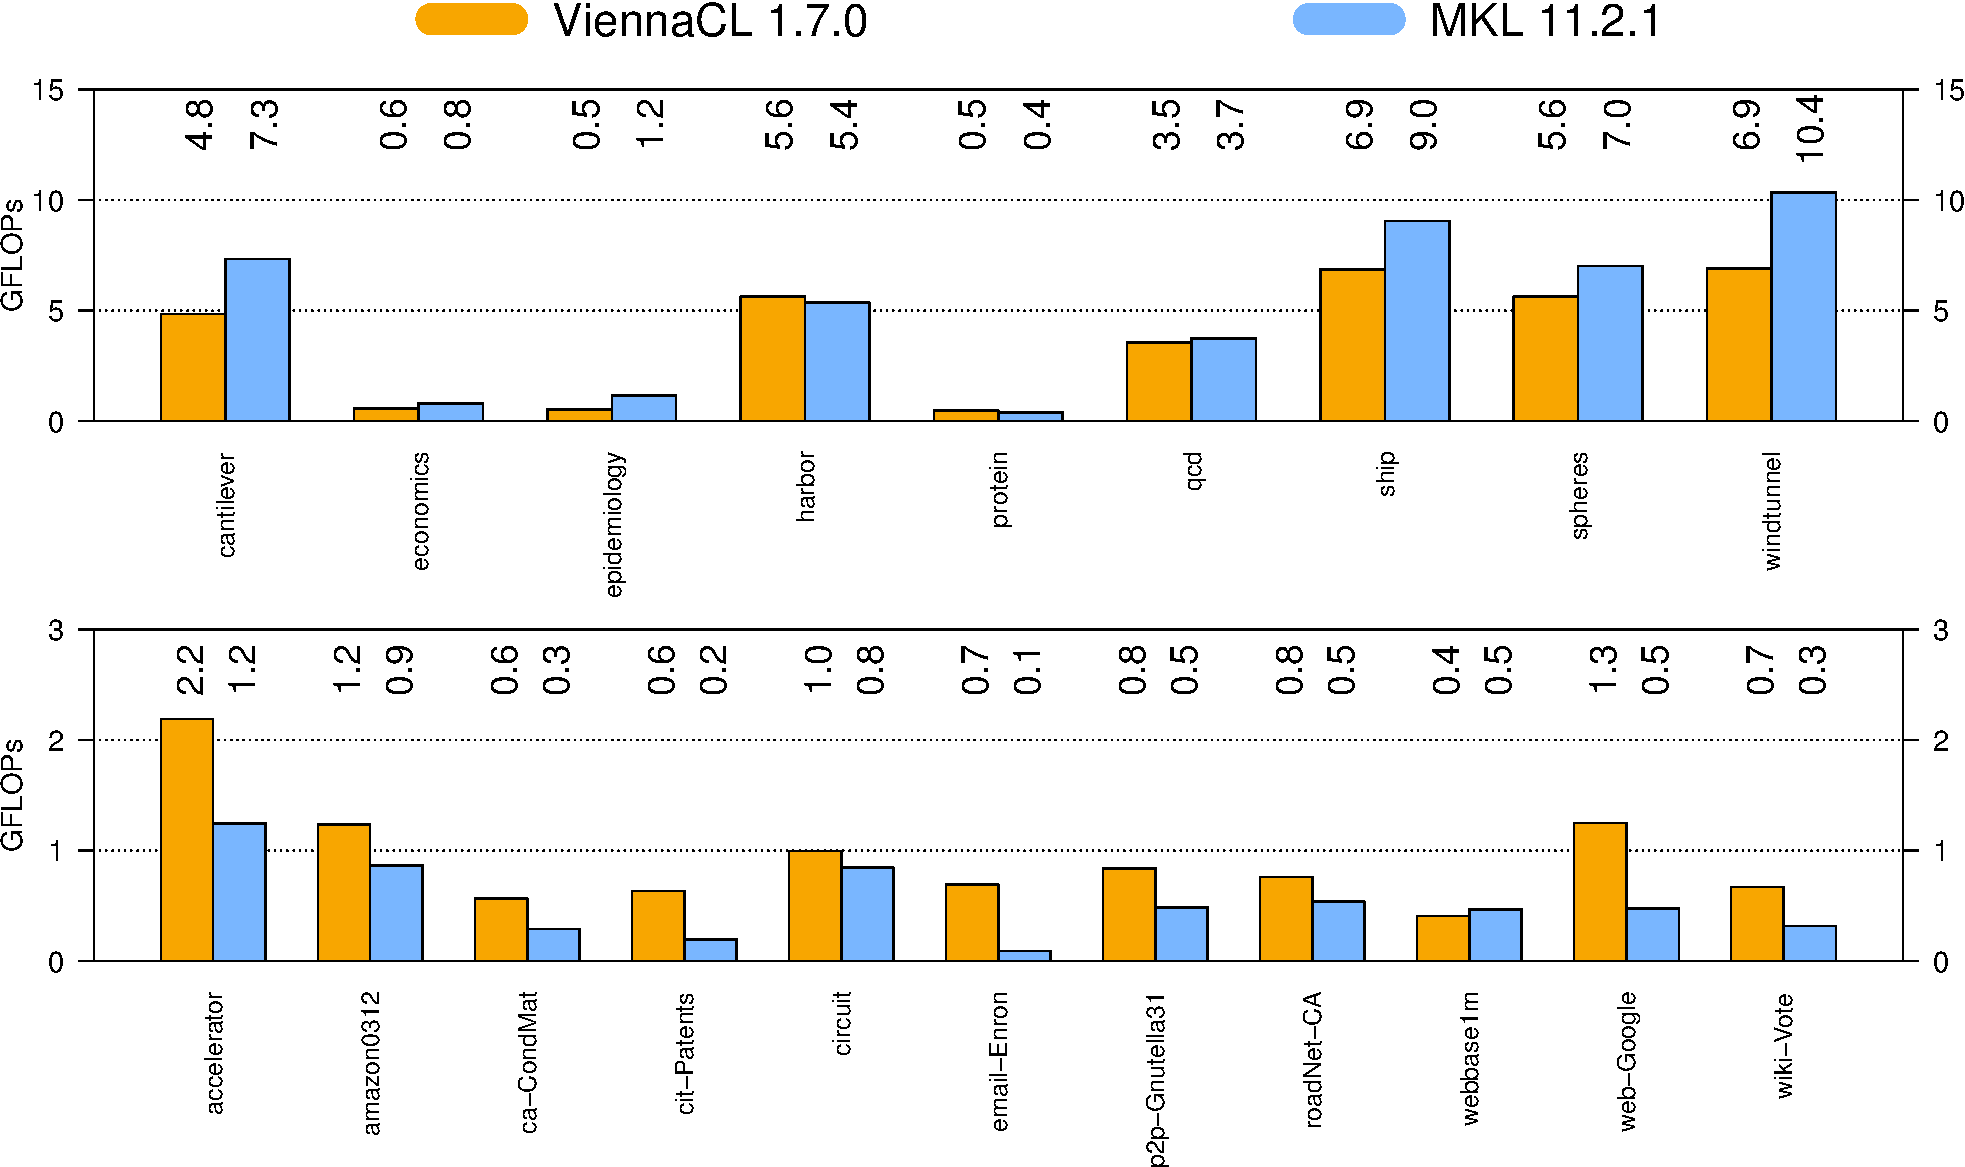
\includegraphics[width=0.999\textwidth]{figures/spgemm_cpu} \\
  Intel Xeon E5-2670v3
 \end{center}
\end{frame}

\begin{frame}{Benchmark Results}
 \begin{center}
  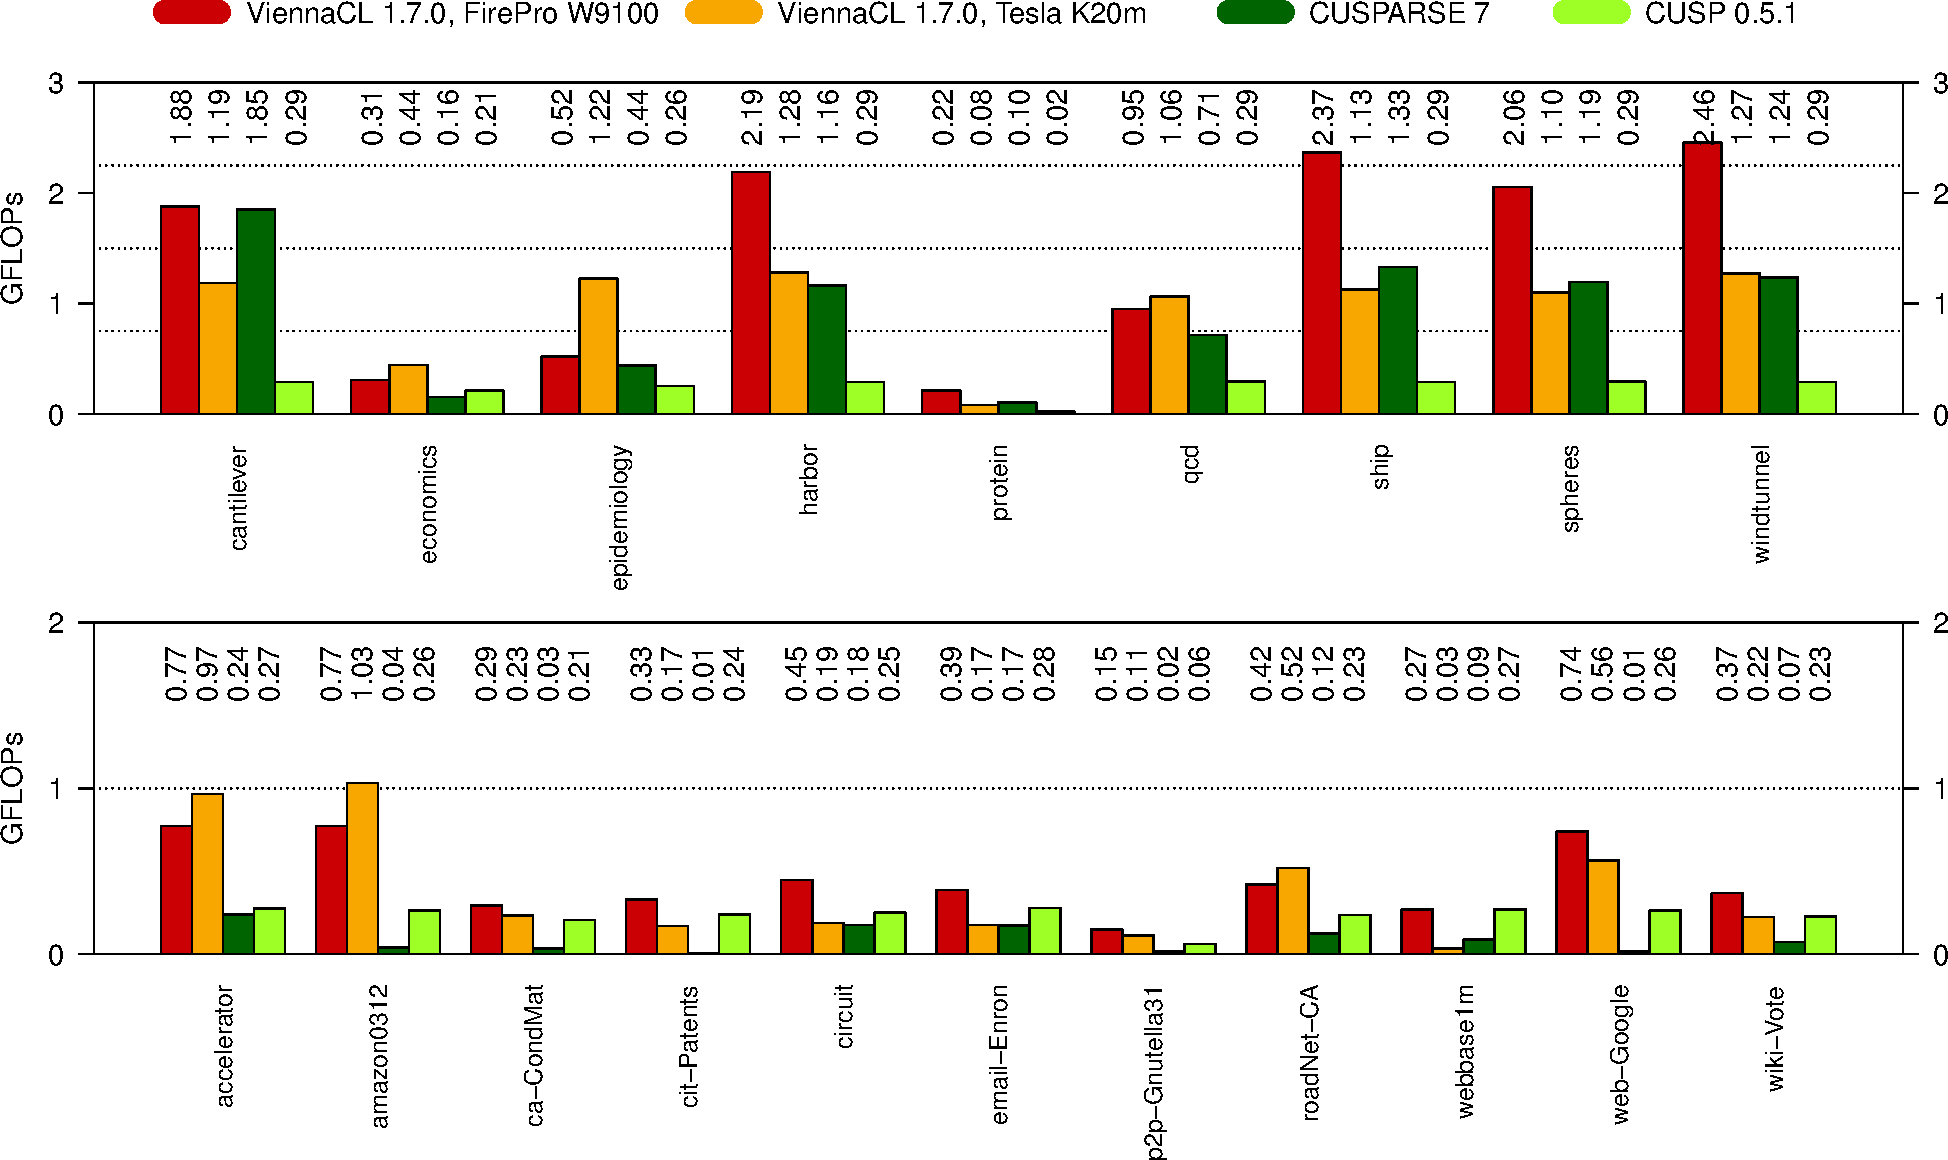
\includegraphics[width=0.999\textwidth]{figures/spgemm_gpu} \\
 AMD FirePro W9100, NVIDIA Tesla K20m
 \end{center}
\end{frame}


\begin{frame}{Benchmark Results}
 \begin{center}
  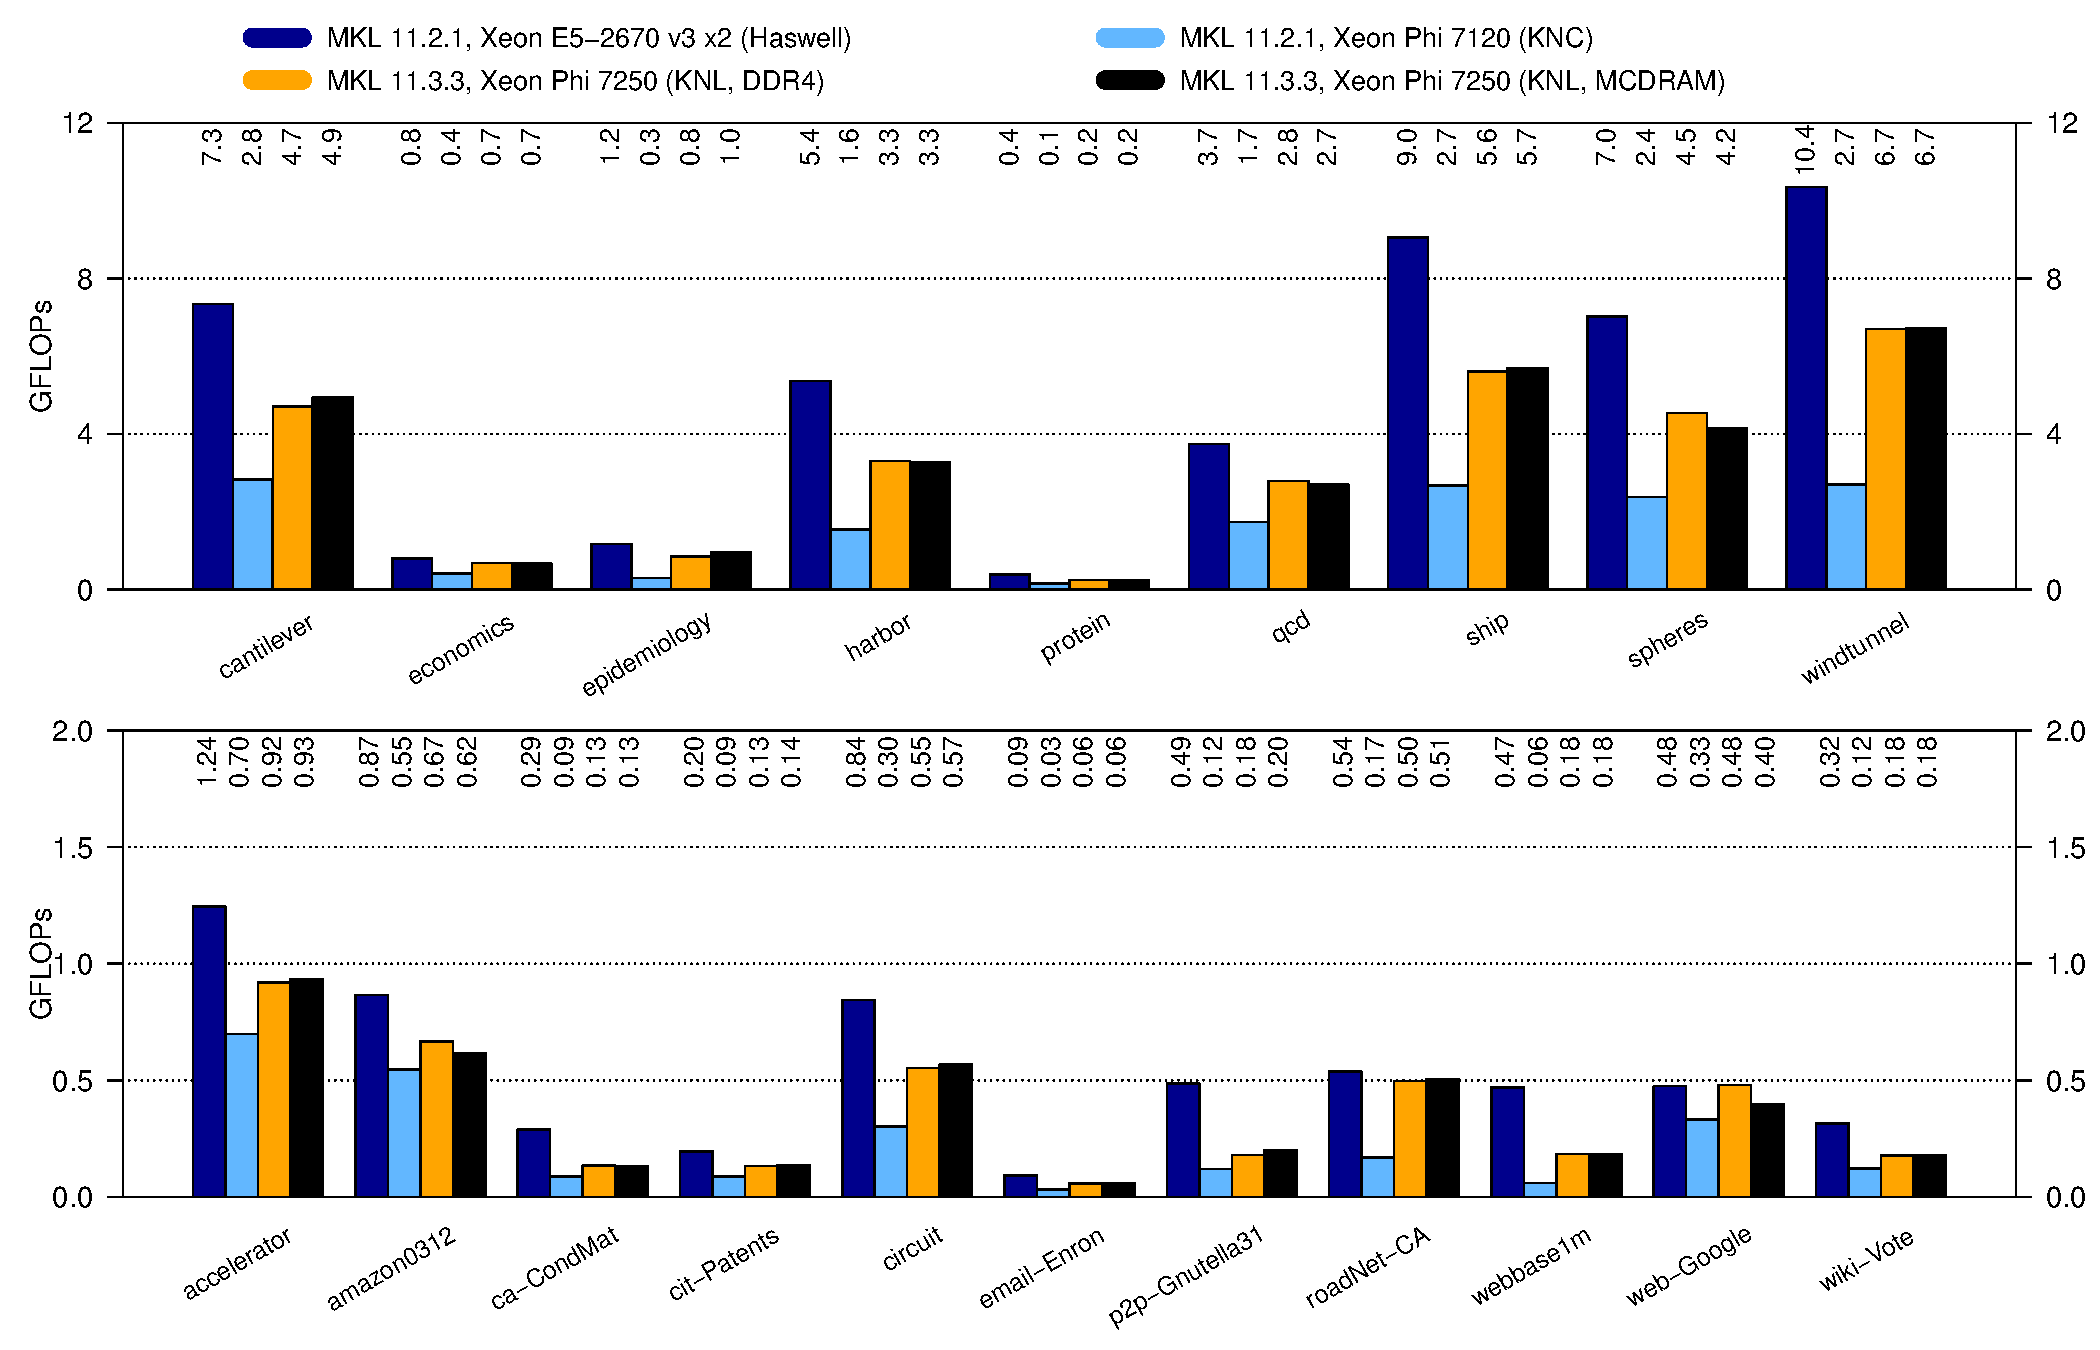
\includegraphics[width=0.999\textwidth]{figures/spgemm-intel} \\
 Comparison on Intel Xeon E5-2670v3 (Haswell) vs. Xeon Phi (KNL)
 \end{center}
\end{frame}

